\chapter{\textit{Phylum Nemathelmintes}}
Los nematodos conforman un clado de animales pluricelulares con forma de gusanos cilíndricos de cuerpo alargado y no segmentado. Carecen de sistema circulatorio y respiratorio y un sistema nervioso simple. Poseen un aparato digestivo completo, compuesto por: boca, esófago, intestino, recto y ano. No son hermafroditas, son dioicos. Poseen ciertas estructuras con valor taxonómico:
\begin{itemize}[itemsep=0pt,parsep=0pt,topsep=0pt,partopsep=0pt]
	\item \textbf{Labios}: estructuras prominentes en número variable que rodean la boca. No presente en todas.
	\item \textbf{Anfidios}: par de depresiones quimiorreceptoras situado a ambos lados del extremo cefálico.
	\item \textbf{Fasmidios}: aberturas situadas en papilas traseras al ano con función olfativa o quimiorreceptora.
	\item \textbf{Alas}: prolongaciones de la cutícula dispuestas en localización cefálica, lateral o caudal.
	\item \textbf{Bolsas copuladoras}: expansión caudal de la cutícula sostenida por costillas de naturaleza muscular situada en el extremo caudal de los machos.
	\item \textbf{Esófago}: puede ser
	\begin{itemize}[itemsep=0pt,parsep=0pt,topsep=0pt,partopsep=0pt]
		\item \textit{Rabditiforme}: generalmente en nemátodos de vida libre, con un itsmo y dos ensanchamientos.
		\item \textit{Estrongiloide}: se ensancha poco a poco.
		\item \textit{Filariforme}: rectilíneo, común en muchos nemátodos.
		\item \textit{Oxiuriforme}: con un estrechamiento y un bulbo posterior.
		\item \textit{Tricuriforme}: formado por un conjunto de células glandulares (esticocitos) que forman el esticosoma. Característico de \textit{Trichuris} y \textit{Trichinella}.
	\end{itemize}
\end{itemize}
\begin{figure}[H]
	\centering
	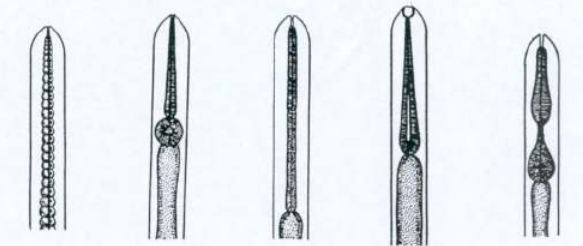
\includegraphics[width=0.8\columnwidth]{figuras/ACV-BioSan-Parasit-NematodosMorf}
	\caption[Morfología de los esófagos de los nemátodos]{Tipos de esófagos de los nemátodos. De izquierda a derecha: tricuriforme, oxiuriforme, filariforme, estrogiloide y rhagditiforme.\label{fig:PARASIT:EsofagosMorf}}
\end{figure}
\subsubsection{\textit{larva migrans} cutanea}
Producida por nemátodos adaptados al ser humano (\textit{Ancylostoma braziliensis}, \textit{A. caninum}, \textit{A. plebotonum}), larvas que se pierden pese a estar adaptadas; y miasis del género \textit{Hypoderma} (ganado vacuno) o \textit{Gasterophilus} (ganado equino). Su diagnóstico es clínico basado en lesiones. Se pueden extraer para su análisis etiológico o mediante tiras para localizar inmunoglobulinas IgE. 
\newpage
\section{Superfamilia \textit{Filaroidea}}
\subsection{\textit{Wachereria bancrofti}}
\subsection{\textit{Dirofilaria inmitis}}
\newpage
\section{Otras familias}
\subsection{\textit{Trichuris trichuria}}
Nemátodo cosmopolita, suele predominar en climas templados y tropicales. Muy común en Asia y Centro y Sudamérica, sobre todo en Brasil. Además, suele coexistir con otros geohelmintos (\textit{Ascaris}, \textit{Enterobius}, etc.) y protozoos (\textit{Giardia}).
\subsubsection{Morfología}
La proción del cuerpo más fina se encuentra ocupada por un esófago tricuriforme, formado por células glandulares superpuestas denominadas esticocitos, formadores del esticosoma, al igual que \textit{Trichinella}.

La hembra es más rectilínea que el macho, que tiene la parte posterior en espiral, donde posee una espícula protegida por una vaina espicular. La hembra posee un ovario y un útero. Los huevos son en forma de huso o limón, con 2 tapones mucosos y en la puesta están sin embrionar. En el exterior se desarrolla la larva L1, que es el agente etiológico.
\begin{figure}[H]
	\centering
	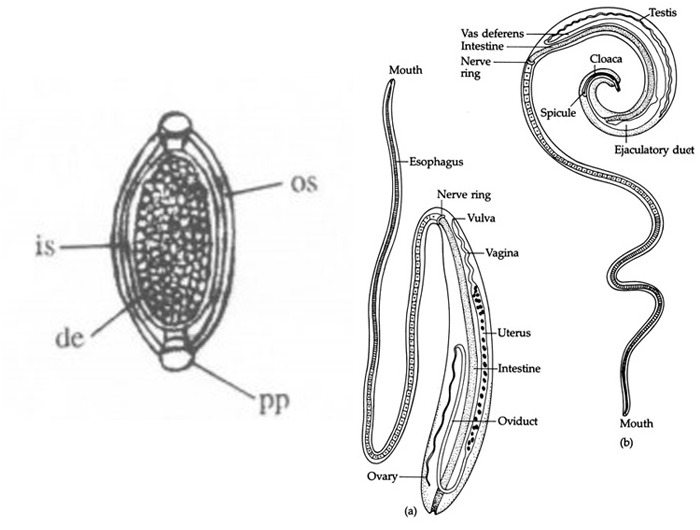
\includegraphics[width=0.6\columnwidth]{figuras/ACV-BioSan-Parasit-TTrichuriaMorf}
	\caption[Morfología de \textit{T. trichuria}]{\textbf{Izquierda}: Huevo de \textit{T. trichuria}, \textbf{OS}: capa exterior; \textbf{IS}: caparazón interior; \textbf{DE}: embrión en desarrollo; \textbf{PP}: papilas polares. \textbf{Centro y derecha}: Fase adulta, \textbf{a)}, hembra; \textbf{b)}, macho \label{fig:PARASIT:TTrichuriaMorf}}
\end{figure}
\begin{multicols}{2}
	\subsubsection{Ciclo biológico}
	Mediante verduras o agua contaminadas con huevos con la larva L1. Los huevos pasan al intestino y en el duodeno se libera la larva L1, dirigiendose a la zona ileoceclar para producirse sucesivas mudas hasta la larva L4 y al fin el adulto, tardando unos 3 meses. En ese momento, machos y hembras copulan y la hembra comienza a eliminar los huevos a razón de 2000 a 20000 por día y hembra. Los huevos salen al exterior mediante las heces y tras unas 2 semanas a una temperatura mayor de 20 C y protegidos de la luz solar, se forma la larva L1, que vuelve a iniciar el ciclo.
	\subsubsection{Control}
	\begin{itemize}[itemsep=0pt,parsep=0pt,topsep=0pt,partopsep=0pt]
		\item Diagnóstico y tratamiento adecuado.
		\item Control de aguas, verduras. Eliminar el hábito de pica. Medidas de higiene
		\item Control de vectores mecánicos como moscas.
	\end{itemize}
	\columnbreak
	\begin{figure}[H]
		\centering
		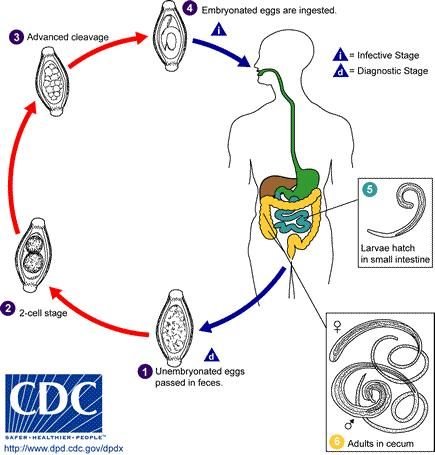
\includegraphics[width=0.95\columnwidth]{figuras/ACV-BioSan-Parasit-TTrichuriaCBios}
		\caption[Ciclo biológico de \textit{T. trichuria}]{Ciclo biológico de \textit{T. trichuria}. Agente: Larva L1 \label{fig:PARASIT:TTrichuriaCBios}}
	\end{figure}
\end{multicols}
\subsubsection{Patogenia}
La tricuriasis tiene un periodo de incubación de 2 a 3 meses, un periodo prepatente de 3 meses y un periodo patente de varios años. Dependiendo de la dosis infectante, puede ser desde asintomática a mortal. Las acciones de \textit{T. trichuria} son:
\begin{itemize}[itemsep=0pt,parsep=0pt,topsep=0pt,partopsep=0pt]
	\item\textbf{Traumática}: en la mucosa, por la presencia de un estilete en la boca que clava en la mucosa y además secreta enzimas proteolíticas con inflamación de mucosa intestinal (llega al sangrado en infecciones masivas) e irritación de plexos nerviosos con hipermotilidad y diarrea.
	\item \textbf{Tóxica}: debido a las sustancias proteolíticas, lo cual se verá mediante la presencia de cristales de Charcot-Leyden en heces, resultado de una eosinofilia.
\end{itemize}
\subsubsection{Sintomatología}
Cursa con dolor abdominal, cefalea, hiperperistaltismo y disenteía y tenesmo. En infecciones masivas (sobre todo en niños), suele cursar con malnutrición que desemboca en anemias, generadas por la acción traumática del adulto que desemboca en malabsorción. La anemia se ve en dedos en palillos de tambor, retraso físico y mental y prolapso rectal.
\subsubsection{Diagnóstico}
\begin{itemize}[itemsep=0pt,parsep=0pt,topsep=0pt,partopsep=0pt]
	\item \textbf{Clínico y etiológico}: si existe prolapso, se pueden observar adultos. Si no, con una colonoscopia. También un síntoma son los dedos en palillos de tambor.
	\item \textbf{Etilológico}: mediante la visión en coprología de cristales de Charcot-Leyden y huevos, dependiendo del número de huevos, se puede ver la masividad de la infección.
\end{itemize}
\newpage
\subsection{\textit{Trichinella spiralis}}
\newpage
\subsection{\textit{Strongyloides stercolaris}}
\textit{Strogyloides stercolaris} es un parásito cosmopolita con alta prevalencia en zonas subtropicales (30 a 100 millones de infectados a nivel global). Son parásitos heterógonos, que alternan vida libre y parásita. Las hembras son partenogenicas\footnote{Hay una hipótesis para explicar la partenogénesis y es la reproducción protándrica: primero se desarrolla una gónada másculina para generar gametos, luego una femenina y se da la autofecundación.} y producen huevos transparentes, ovalados y con opérculo.
\subsubsection{Morfología}
\begin{itemize}[itemsep=0pt,parsep=0pt,topsep=0pt,partopsep=0pt]
	\item \textbf{Vida libre}: tienen una representación cromosómica haploide (machos) o diploide (hembras). Presentan un esófago rabditoide con una protursión prebulbo y una vulva dispuesta anteriormente. Las hembras de vida libre son más pequeñas y ponen más huevos que las parásitas, ya que poseen dos ovarios y dos úteros (frente al único ovario y útero de las parasitarias). Anfidelfas, un útero va a posterior (asociado a la puesta de huevos) y otro anterior. En el propio útero se desarrollan hasta la primera fase larvaria (L1). Posteriormente desarrollan un esófago rabdiforme y continuan su ciclo (L1r\footnote{r por su tipo de esófago, rabdiforme; frente a f, filariforme}, L2r, L3f, L4) fuera del útero.
	\item \textbf{Vida parásita}: presentan una dotación cromosómica triploide, en el caso de las hembras. Son también anfidelfas y presentan una esófago filariforme. Presentan un ciclo vital similar al anterior, pero sin fase L4.
\end{itemize}
\subsubsection{Ciclo biológico}
El ciclo vital puede ser:
\begin{itemize}[itemsep=0pt,parsep=0pt,topsep=0pt,partopsep=0pt]
	\item \textbf{Indirécto o heterogónico}: fases de vida libre.
	\item \textbf{Dirécto u homogónico}: en sus fases de vida parásita. El individuo avanza en su ciclo vital hasta la fase L3r y se produce una penetración al hospedador via subcutánea, transplacentaria, galactógena u oral.
\end{itemize}

Cuando la larva L3f penetra por la piel del hospedador definitivo, se desplaza por el sistema linfático y el torrente sanguíneo hasta las arterias pulmonares. Sigue avanzando hasta que rompe capilares y accede al espacio alveolar. Una vez allí, asciende por la tráquea hasta que es deglutida. En el intestino, la larva L3f se transforma en L4f y pasa a la adultez. Allí, tendrá lugar la partenogénesis y pondrá huevos saliendo la larva L1r en su interior. Los que tengan dotación cromosómica n o 2n, saldrán al exterior y seguirán un ciclo de vida indirecto o, en el caso de las larvas triploides, eclosionarán en el intestino, pudiendo:
\begin{itemize}[itemsep=0pt,parsep=0pt,topsep=0pt,partopsep=0pt]
	\item \textbf{Endoautoinvasión}: muda a L2r y a L3f y vuelve al torrente sanguíneo atravesando el intestino.
	\item \textbf{Migración a zona perianal}: se produce una muda a L2r y a L3f. Muchas de estas se caen del individuo contaminando el suelo permitiendo la infección de otros individuos (no humanos incluidos). Otras intentan penetrar por la piel (exoautoinvasión), en un fenómeno conocido como erupción reptante perianal. Los túneles subcutáneos son muy característicos, observándose un extremo vesiculoso que marca el avance de la larva, y el resto seco y duro. Remitirá a las dos o tres semanas. La larva L3f cerraría el ciclo.
\end{itemize}
\begin{multicols}{2}
	\begin{figure}[H]
		\centering
		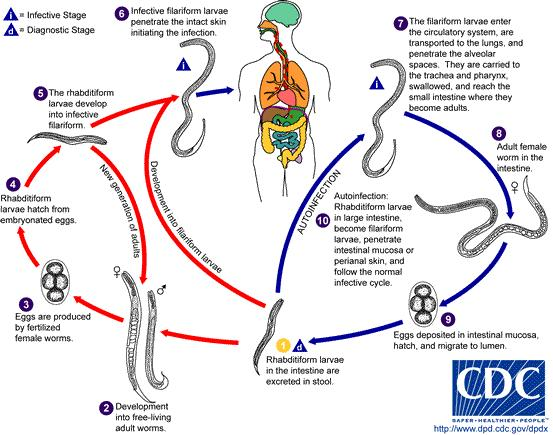
\includegraphics[width=0.9\columnwidth]{figuras/ACV-BioSan-Parasit-SStercolarisCbios}
		\caption[Ciclo vital de \textit{S. stercolaris}]{Ciclo vital de \textit{S. stercolaris}. Agente: Larva L3f.\label{fig:PARASIT:SStercolarisCBios}}
	\end{figure}
	\begin{figure}[H]
		\centering
		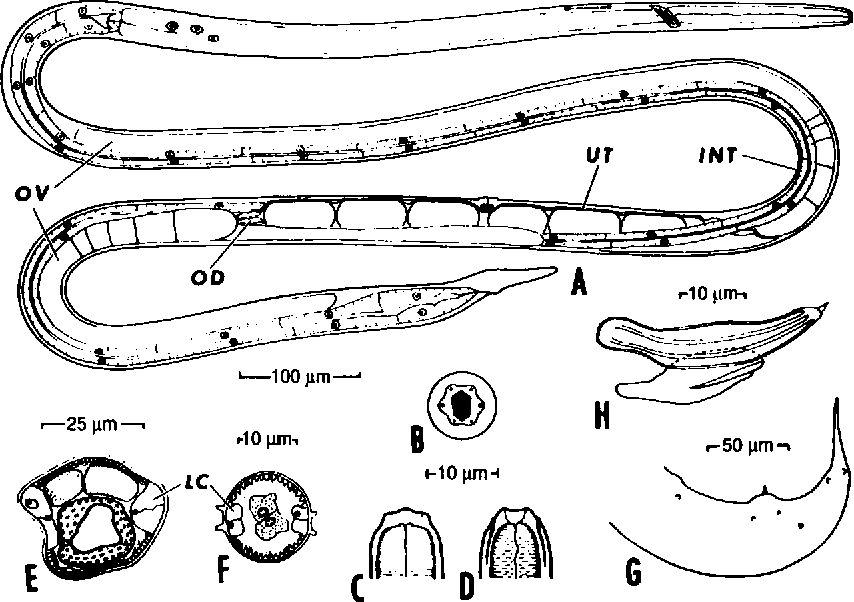
\includegraphics[width=0.9\columnwidth]{figuras/ACV-BioSan-Parasit-SStercolarisMorf}
		\caption[Morfología de la forma parásita de \textit{S. stercolaris}]{Morfología de la forma parasitaria de \textit{S. stercolaris}. \textbf{A}: Visión lateral de una hembra parasitaria (OV: ovario, OD: oviducto, UT: útero, INT: intestino); \textbf{B}: vista anterior apical; \textbf{C}: Vista posterior lateral; \textbf{C}: Vista posterior dorsal; \textbf{E}: Sección a nivel del ovario (LC: cordón lateral); \textbf{F}: Sección intestinal de la larva filariforme; \textbf{G}: vistal de la cola de macho de vida libre; \textbf{H}: Espícula derecha bajo la línea del gobernáculo.\label{fig:PARASIT:SStercolarisMorf}}
	\end{figure}
\end{multicols}

\subsubsection{Patogenia}
El periodo de incubación es de unas dos semanas y el prepatente de 2 a 3 semanas.
\begin{itemize}[itemsep=0pt,parsep=0pt,topsep=0pt,partopsep=0pt]
	\item \textbf{Fase invasiva}: la larva L3f penetra por la piel. Se da una acción traumática y vehiculizadora de bacterias procedentes del interior (microbiota intestinal) o del exterior (suelo), generando hinchazón en el punto de la picadura, prurito local y \textit{larva migrans} cutánea.
	\item \textbf{Fase pulmonar}: acción traumática (ruptura de capilares) y vehiculadora. Causa hemorragias, síntomas asmáticos, tos seca e improductiva, dolor en el pecho, etc. que pasan desapercibidos salvo si se cursa una neumonía bacteriana.
	\item \textbf{Fase intestinal}: acción traumática de la L4f y de los adultos en las vellosidades. Producen un fuerte y punzante dolor epigástrico y diarreas que se exacerban con el consumo de corticoides con parasitaciones masivas.
\end{itemize}
\subsubsection{Diagnosis}
\begin{itemize}[itemsep=0pt,parsep=0pt,topsep=0pt,partopsep=0pt]
	\item \textbf{Etiológico}: en pequeñas infestaciones, mediante el método de concentración de Baermann, que concentra con hidro y termotropismo positivo a la larva y la deja flotando en una solución de ZnS$o_4$. Se ha visto que las hembras son capaces de producir huevos en alveolos pulmonares, por lo que se pueden ver en aspirados pulmonares hembras adultas, huevos y larvas L3f.
	\item \textbf{Indirecto}: muy útil en las primeras fases en las que el parásito se encuentra en la sangre. Mediante ELISA o IFI se pueden ver, pero producen reacciones cruzadas con los ancilostómidos.
\end{itemize}
\newpage
\subsection{\textit{Ancylostoma duodenale} y \textit{Necator americanus}}
\subsubsection{Morfología y localización}
\begin{multicols}{2}
	\subsubsection*{\textit{Ancylostoma duodenale}}
	\textit{Angylostoma duodenale} es una uncinaria del Viejo Mundo. Presenta una cápsula con dientes (4 superiores y dos en la base) con los que cortan las microvellosidades. Los machos son más pequeños que las hembras. En sus glándulas esofágicas presentan sustancias anticoagulantes que permiten la salida de sangre, lo que llevará el desarrollo de anemias por la pérdida de sangre. Las larvas son hematófogas y los adultos se alimentan de plasma, que llegan a obtener el 50 \% del hierro reducido perdido.
	
	Presentan un esófago estrongiliforme, muy musculoso, ligeramente más ensanchado en posterior. Las hembras son anfidelfas y ovíparas, liberan sus huevos en estado de mórula. Los machos presentan bolsa copuladora con tres lóbulos y costillas laterales separadas. Las espículas también están separadas. La larva L3 posee una punta muy puntiaguda y madura a 22 grados.
	\columnbreak
	\subsubsection*{\textit{Necator americanus}}
	\textit{Necator americanus} es la uncinaria del Nuevo Mundo. Posee una cápsula con 2 placas cortantes en la parte superior y dos dientes en la parte inferior.  Al igual que los \textit{Ancylostomas}, los machos son más pequeños que las hembras (anfidelfas y ovíparas, que eliminan huevos en forma de mórula), y poseen esófagos estrongiloides con glándulas secretoras de anticuagulantes.
	
	Los machos poseen bolsas copuladoras  con tres lóbulos y costillas laterlaes semifusionadas. Las espículas se fusionan en la punta y la larva L3 termina en punta roma. Mudan a 28 - 32 grados.
\end{multicols}
\vspace*{-1cm}
\begin{figure}[H]
	\centering
	\subfigure[Morfología de \textit{A. duodenale}]{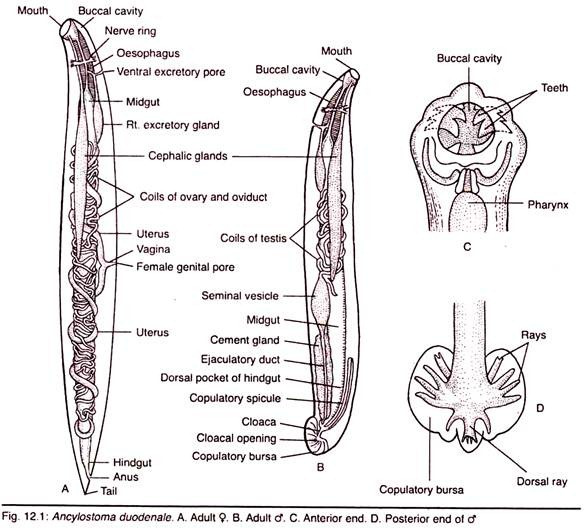
\includegraphics[width=0.475\columnwidth]{figuras/ACV-BioSan-ParasitAduodenaleMorf}}
	\subfigure[Diferencias morfológicas entre \textit{A. duodenale} y \textit{N. americanus}]{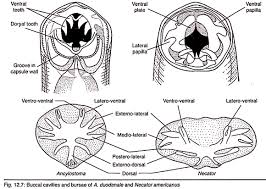
\includegraphics[width=0.475\columnwidth]{figuras/ACV-BioSan-ParasitAduodenaleNamericanusMorf}}
	\caption[Morfología de \textit{A. duodenale} y \textit{N. americanus}]{Morfología de \textit{A. duodenale} y \textit{N. americanus} y sus diferencias más notables.}
\end{figure}
\subsubsection{Ciclo biológico}
La vía de infección es percutánea, aunque \textit{Ancylostoma duodenale} pueden infectar por vía oral, transplacentaria o galactógena.

El ciclo comienza con las larvas L3, que mediante su geotropismo negativo y fototropismo y termotropismo positivos, localizan un animal y penetran por la piel de zonas de los pies, al disponerse como agujas en posición vertical. En este contexto, alguna larvas L3 se pierden por la piel y forman el síndrome de la \textit{larva migrans} subcutánea. Una vez en el organismo, la larva L3 viaja por el sistema circulatorio hasta el corazón y las arterias pulmonares para salir por ellos y ser deglutidos al subir por la faringe. Una vez deglutidas, la larva L3 muda a L4 a los 5 días y a adulto a las 8 semanas. En ese momento se da la reproducción, expulsandose los huevos embrionados en forma de mórula. Tras 7 días, eclosiona la larva L1, que muda en el exterior a L2 y L3. Así mismo, \textit{A. duodenale} es capaz de quedarse latente en distintos tejidos e infectar mediante huevos embrionados o ingestión de larva L3.

Tiene como reservorios el cerdo, los perros y las vacas.
\begin{figure}[H]
	\centering
	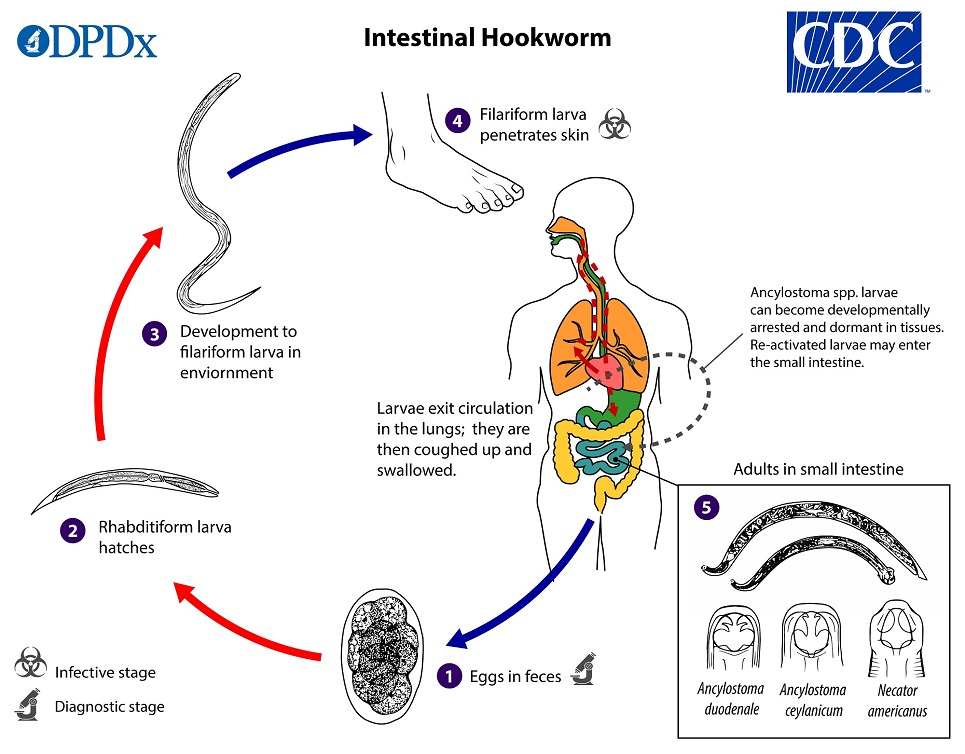
\includegraphics[width=0.7\columnwidth]{../Parasitologia/A.README/figuras/ACV-BioSan-ParasitAduodenaleNamericanusCBios}
	\caption[Ciclo vital de \textit{A. duodenale} y \textit{N. americanus}]{Ciclo vital de \textit{A. duodenale} y \textit{N. americanus}. Agente: Larva L3f.\label{fig:PARASIT:AduodenaleNamericanusCBios}}
\end{figure}
\subsubsection{Patogenia y sintomatología}
La uncinariosis, su gravedad, depende, del número de parásitos, la duración del periodo patente (antes de aplicar tratamientos) y el estado nutricional, fisiológico e inmunológico del infectado. El periodo de incubación es de 4 horas, el prepatente de 5 a 6 semanas y el patente de hasta 20 años. Las uncinarias segregan distitnas moléculas que inhiben o antagonizan con la respuesta inmune. En cuanto a síntomas y daños:
\begin{itemize}[itemsep=0pt,parsep=0pt,topsep=0pt,partopsep=0pt]
	\item\textbf{Fase invasiva}: se produce urticaria y adenopatías en los ganglios cercanos, que siguen presentes durante toda la enfermedad. La inflamación ganglionar es indolora y los gánglios, móviles.
	\item\textbf{Fase pulmonar}: si la parasitosis es masiva, por la acción vehiculizadora pueden producir neumonías y pequeñas hemorragias. Generan una eosinofilia importante. Generan tos seca e improductiva.
	\item\textbf{Fase intestinal}: la larva L3 se alimenta de sangre, se reabsorben el 50 \% del hierro que estas toman. Las infecciones tienden a la cronificación y llevar a anemias. Los niveles de albúmina descienden a valores mínimos con resecación de piel y pelo. El dolor abdominal es insidioso, intermitente y ligero. Puede producirse anorexia y deposiciones con sangre. En niños puede provocar retraso mental y retardo en la pubertad.
\end{itemize}
\subsubsection{Diagnóstico}
\begin{itemize}[itemsep=0pt,parsep=0pt,topsep=0pt,partopsep=0pt]
	\item\textbf{Etiológico} mediante coprología se pueden ver huevos ovalados, transparentes y sin larvas en su interior.
\end{itemize}
\newpage
\subsection{\textit{Ascaris lumbricoides}}
Nemátodo cosmopolita, con mayor frecuencias en zonas tropicales y templadas. Tiene prevalencias mundiales de unos 1000 millones de personas, con unas 20 mil muertes anuales. Fue uno de los primeros parásitos en conocerse, debido a su enorme tamaño: los machos rondan los 15 a 30 cm y las hembras de 20 a 40.
\subsubsection{Morfología}
Machos y hembras poseen una boca con tres grandes labios, los cuales están rodeados de dentículos que, en \textit{A. lumbricoides} son cónicos, pero que en \textit{A. suum}\footnote{Parásitos de cerdos} son aplanados. Su esófago es estrongiliforme o en forma de mazo. Los machos no tiene bolsa copuladora, pero sí dos espículas iguales y anchas con las que penetra en la vulva y facilita la cópula. Poseen numerosas papilas anales y postanales. Las hembras presentan la vulva en el tercio anterior del cuerpo, 2 ovarios y 2 úteros enrollados sobre el intestino, los cuales pueden contener hasta 27 millones de huevos.

Los huevos son de color amarillo-marrón y son muy resistentes a los ácidos gracias a tres capas: una externa albuminoide (en pegotes); una media quitinosa y una intern lipídica, la cual le confiere una gran resistencia. Si el huevo está sin embrionar es de forma más alargada y estrecha, y si está embrionado (que son los que elimina la hembra) es redondo. El agente etiológico es el huevo con la larva L3 en su interior.
\subsubsection{Ciclo biológico}
Comienza con la ingestión de alimentos, agua o tierra contaminados con huevos con L3. Atraviesan el estómago y en el duodeno eclosionan, liberando a la L3, que atraviesa la mucosa intestinal y pasa a un capilar sanguineo, mediante el cual llega a la aorta y de ahí a los pulmones. rompiendo los capilares pulmonares, sale al espacio alveolar y ahí provoca que L3 suba por la tráquea para ser deglutida, volviendo al intestino. Allí, se transforma en L4 y en adulto. En unos 20 días tras la ingestión, las larvas L3 están en el pulmón, en unos 30 se transforman en adultos y en 2 meses eliminan huevos, que tras dos semanas a temperaturas templadas y en oscuridad, se transforman en L3.
\subsubsection{Control}
\begin{itemize}[itemsep=0pt,parsep=0pt,topsep=0pt,partopsep=0pt]
	\item Correcto saneamiento de las aguas, control de las heces y buenas prácticas higiénicas.
	\item Correcto diagnóstico y tratamiento en personas parasitadas.
\end{itemize}
\begin{multicols}{2}
	\begin{figure}[H]
		\centering
		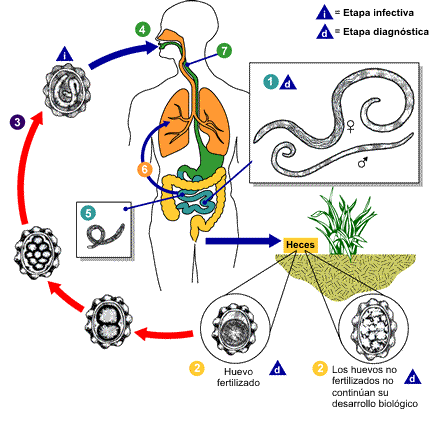
\includegraphics[width=0.9\columnwidth]{figuras/ACV-BioSan-Parasit-ALumbricoidesCBios}
		\caption[Ciclo vital de \textit{A. lumbricoides}]{Ciclo vital de \textit{A. lumbricoides}. Agente: Larva L3f.\label{fig:PARASIT:AlumbricoidesCBios}}
	\end{figure}
	\columnbreak
	\begin{figure}[H]
		\centering
		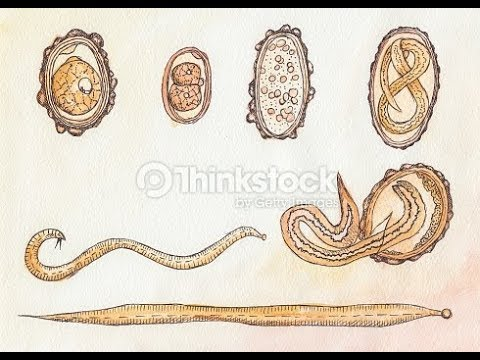
\includegraphics[trim=0 0.5cm 0 0.5cm,clip,width=\columnwidth]{figuras/ACV-BioSan-Parasit-ALumbricoidesMorf}
		\caption[Morfología de \textit{A. lumbricoides}]{Morfología de \textit{A. lumbricoides}. En la parte superior, las diferente fases del huevo hasta la formación de la larva L1; en la parte media, un macho y el momento de la salida de la larva L1 del huevo; parte inferior, una hembra.\label{fig:PARASIT:AlumbricoidesMorf}}
	\end{figure}
\end{multicols}
\subsubsection{Patogenia}
La ascariasis produce las siguientes acciones:
\begin{itemize}[itemsep=0pt,parsep=0pt,topsep=0pt,partopsep=0pt]
	\item\textbf{Traumática}: por parte de la larva L3 por la ruptura de capilares pulmonares. Cuando la infección es masiva y se presenta con fiebre, ésta provoca la movilización de los adultos, que intentan escapar por los orificios del cuerpo, normalmente ano, pero también nariz, ojo, oído o boca, produciéndose acciones traumáticas.
	\item\textbf{Vehiculadora}: de larva L3 mediante el transporte de bacterias del intestino al pulmón.
	\item\textbf{Mecánica}: de obstrucción de los adultos en el intestino.
	\item\textbf{Expolidora y tóxica}: por parte de los adultos.
\end{itemize}
\subsubsection{Sintomatología}
El periodo de incubación es variable y depende del grado de parasitación desde 7 días en infestaciones masivas con síntomas pulmonares a 2 meses cuando hay problemas intestinales. El periodo prepatente es de 60 días y el patente puede extenderse durante años.

Las larvas producen inflamaciones por acción vehiculizadora, hemorragias en pulmón y edema. Con infecciones secundarias, se producen infiltrados de células epiteliales y glóbulos blancos y neumonía conocidos como síndrome de Loëfler que puede llevar a la muerte. Los adultos en el intestino producen enteritis (dolores intestinales), desnutrición y malabsorción de lactosa con pérdida apetito y peso, obstrucción intestinal y de conductos de glándulas anejas, fenómenos de sensibilización (prurito, urticaria, edema facial, insomnio) y eosinofilia en sangre. Los adultos errantes producen una fuerte acción traumática en su recorrido por su tamaño.
\subsubsection{Diagnóstico}
\begin{itemize}[itemsep=0pt,parsep=0pt,topsep=0pt,partopsep=0pt]
	\item\textbf{Etiológico}: por coprología, observando huevos a los dos meses de la infección, u observando larvas L3 en esputos o lavados gástricos.
	\item \textbf{Clínico}: por radiografía con la que se pueden ver las infecciones de un solo sexo.
	\item \textbf{Indirecto}: ELISA, RIA,$\dots$ en los periodos prepatentes (existen larvas L3 en sangre y producen una gran estimulación antigénica).
\end{itemize}
\newpage
\subsection{\textit{Enterobius vermicularis}}
Nemátodo parásito cosmopolita, predomina más en climas templados que en tropicales y aunque tiene una gama amplia de hospedadores definitivos, no se encuentra en perros o gatos. La incidencia en España es de unos 250 casos diagnosticados al año, no siendo cifras reales.
\subsubsection{Morfología}
Machos y hembras tienen el esófago oxiuriforme (con un bulbo) y en la parte anterior alas cefálicas. Las hembras miden entre 8 y 13 mmm, poseen 2 ovarios con dos úteros y una cola muy larga y puntiaguda denominada alfiler. Los machos miden entre 2 y 5 mm, con cola curvada y alas caudales. No tienen bolsa copuladora pero sí una espícula y unas papilas pre y poscloacales. No tienen gobernáculo.

Los huevos son transparentes, con uno de los lados más aplanado. Son muy ligeros, por lo que pueden estar suspendidos en el aire unos 2 minutos. Gozan de gran resistencia, pueden permanecer latentes hasta dos meses y son inmunes a insecticidas caseros. Los huevos que pone la hembra están embrionados con la larva L1.
\begin{figure}[H]
	\centering
	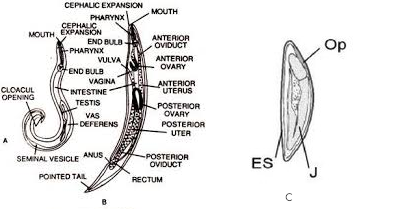
\includegraphics[width=0.8\columnwidth]{figuras/ACV-BioSan-Parasit-EVermicularisMorf}
	\caption[Morfología de \textit{E. Vermicularis}]{Morfología de \textit{E. Vermicularis}.\textbf{A}: Macho; \textbf{B}: Hembra; \textbf{C}: Huevo, \textbf{OP}: opérculo, \textbf{ES}: capa externa, \textbf{J}: embrión \label{fig:PARASIT:EVermicularisMorf}}
\end{figure}
\vspace*{-1cm}
\subsubsection{Ciclo biológico}
\begin{multicols}{2}
	Comienza con la ingestión de alimentos o agua contaminados con huevos con la larva L2 o mediante inhalación y posterior deglución. En el intestino eclosiona el huevo, liberando la larva L2, que avanza por el intestino hasta la zona ileocecal, donde muda a larva L3, luego a larva L4 y posteriormente a adulto. Algunos adultos se alojan en el apéndice, por lo que pueden generar apendicitis. Machos y hembras copulan en la región ileocecal y se realiza la puesta de huevos tras dos mese. Los huevos no se eliminan por las heces, si no que al anochecer, la hembra viaja a los bordes perianales y pone allí los huevos. Si caen al exterior, necesitan un tiempo a una temperatura de 22 C para que mude la larva de L1 a L2. Si se quedan en la zona perianal, en unas 4 horas se produce la muda de L1 a L2. Las hembras, al movilizarse, provacan prurito anal, que al rascarse se quedan los huevos en las uñas y pueden llegar otra vez al intestino.
	\columnbreak
	\begin{figure}[H]
		\centering
		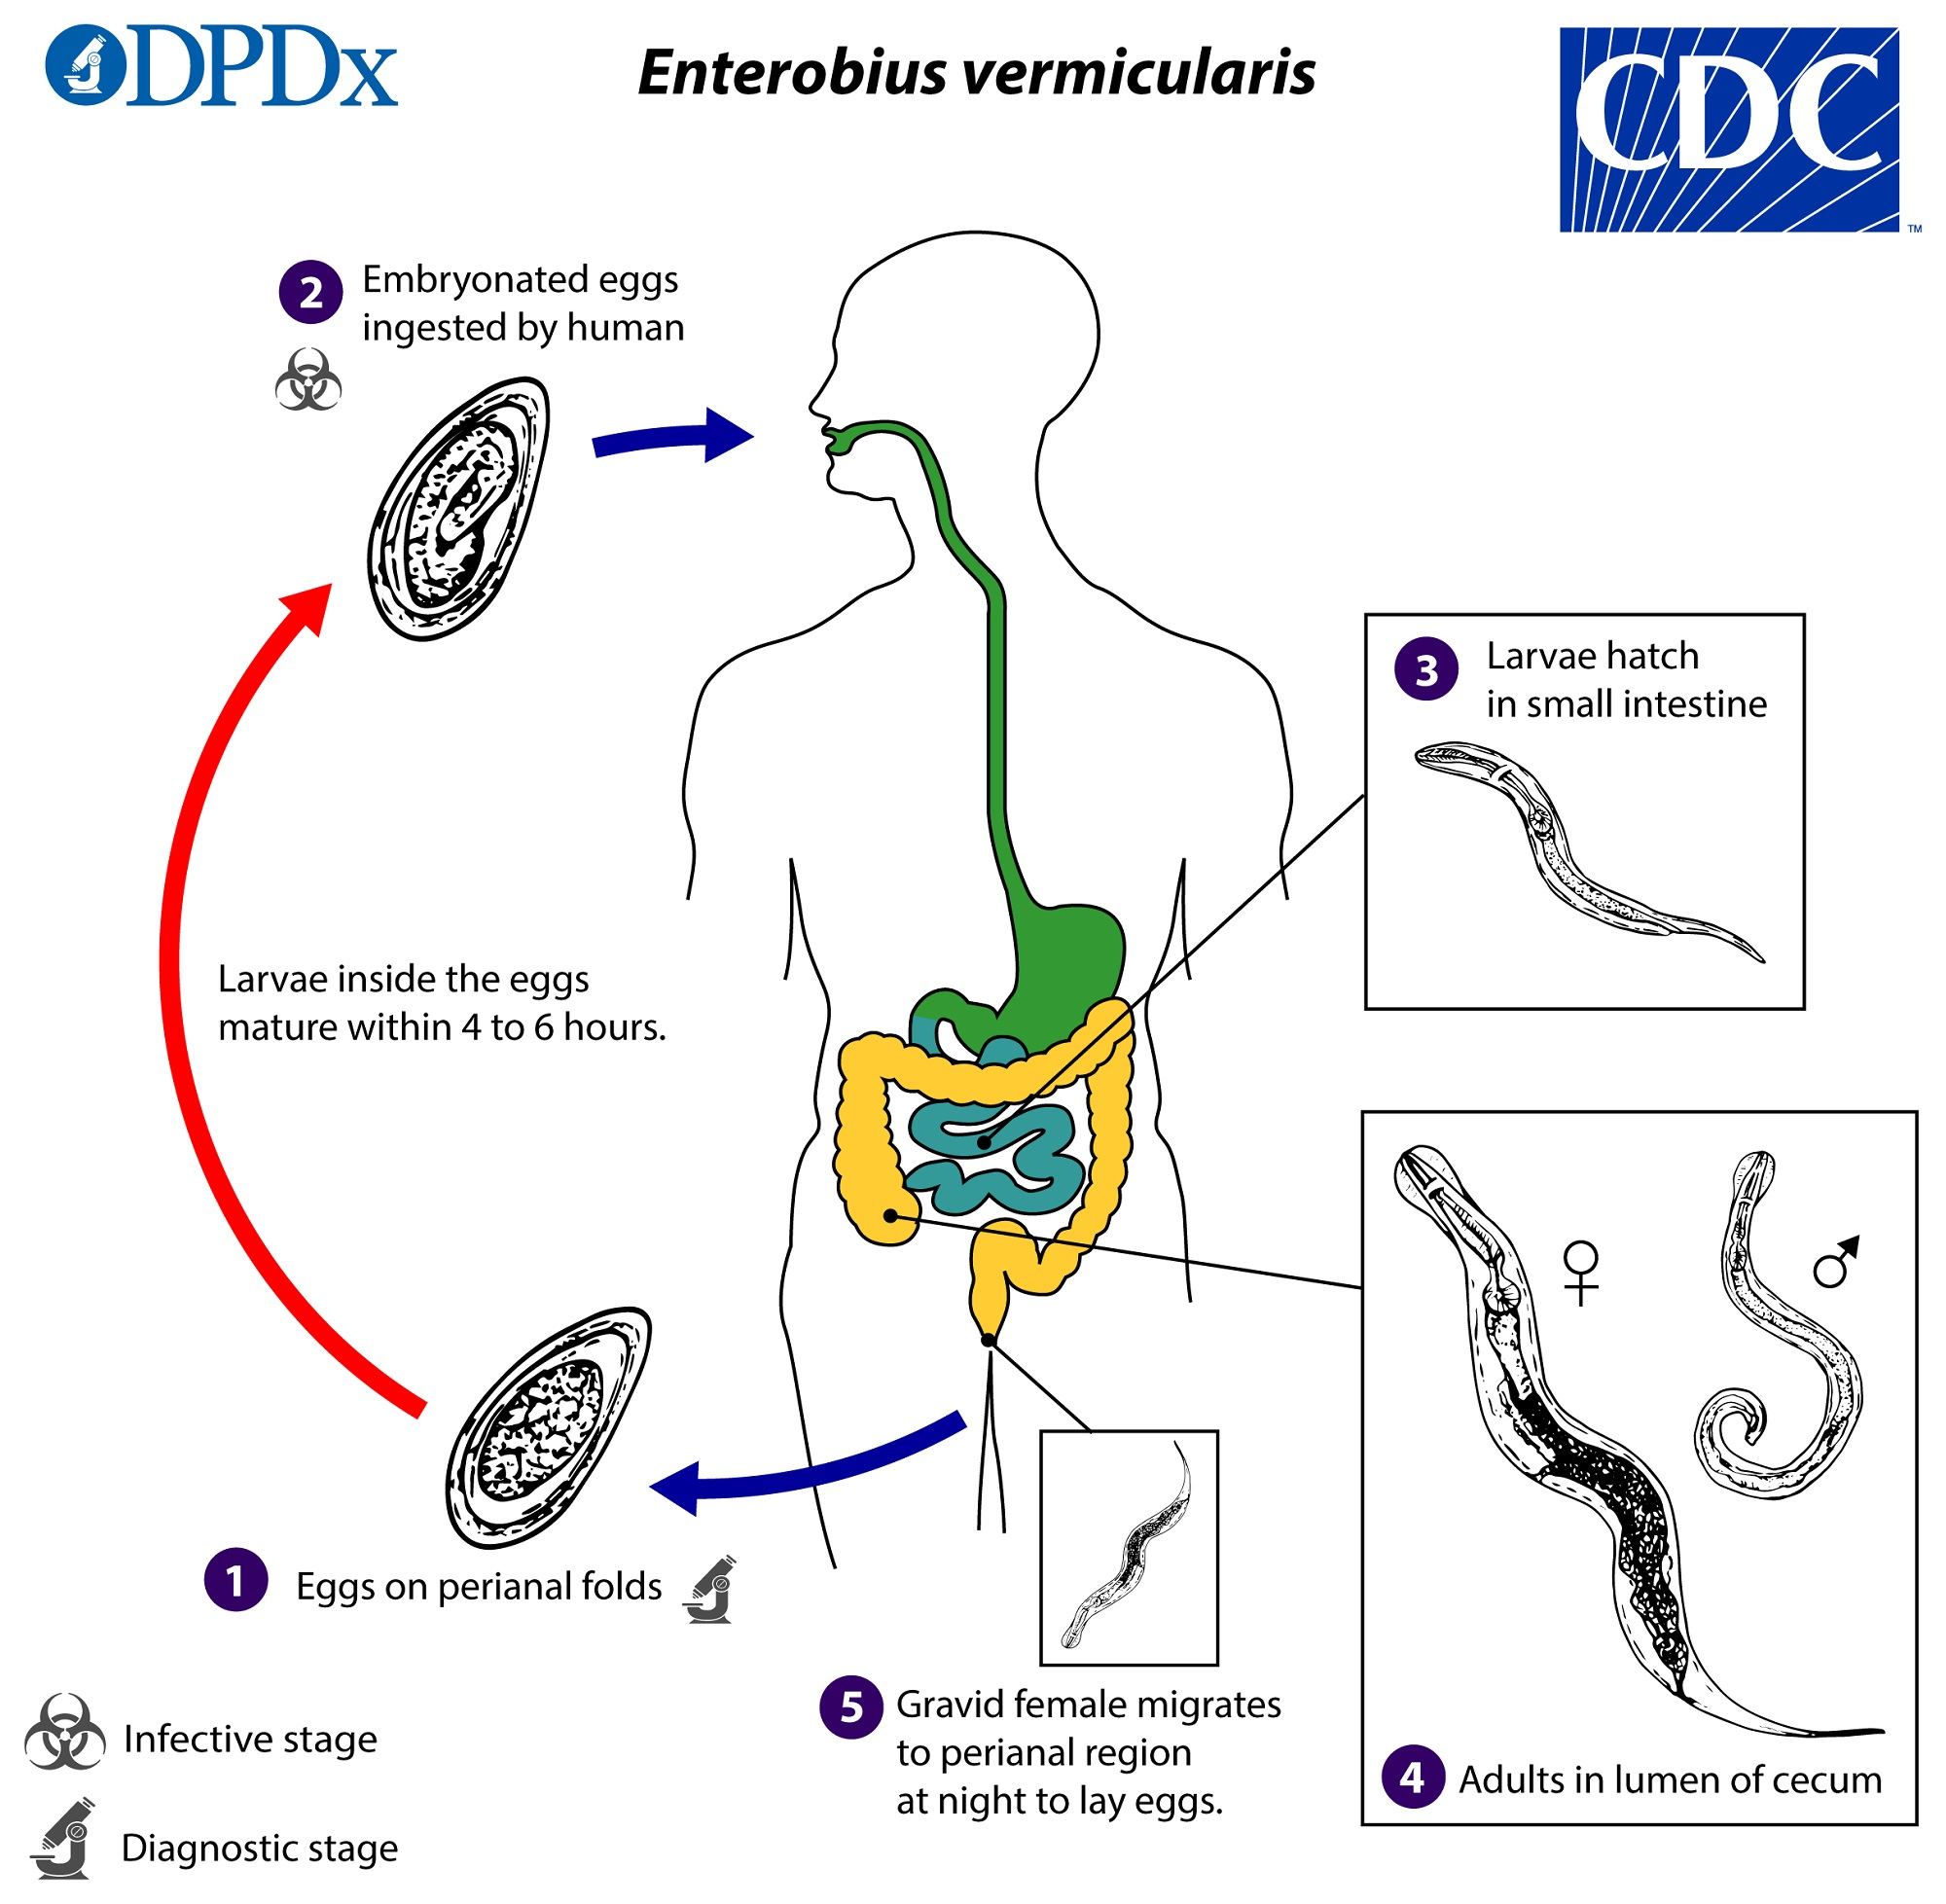
\includegraphics[width=\columnwidth]{figuras/ACV-BioSan-Parasit-EVermicularisCBios}
		\caption[Ciclo vital de \textit{E. Vermicularis}]{Ciclo vital de \textit{E. Vermicularis}. Agente: Larva L2.\label{fig:PARASIT:EVermicularisCBios}}
	\end{figure}
\end{multicols}
Así, las vías de infección son:
\begin{itemize}[itemsep=0pt,parsep=0pt,topsep=0pt,partopsep=0pt]
	\item\textbf{Retroinfestación}: se produce cuando en la zona perianal eclosiona el huevo y la larva L2 vuelve por el ano al intestino, produciendose las mudas hasta llegar a la madurez.
	\item\textbf{Autoinfestación exógena}: mediante via ano-mano-boca.
	\item\textbf{Inhalación}: mediante el movimiento de objetos (sabanas, etc.) con huevos.
	\item\textbf{Ingestión}: por mala higiene y consumo de alimentos contaminados.
\end{itemize}
\subsubsection{Control}
El control se debe hacer a nivel de huevos, pues en cuanto hay un miembro de la familia parasitado, es muy fácil su contagio al resto. Se debe hacer analisis coprológico, tener cuidado al limpiar objetos, buenos hábitos de higiene.
\subsubsection{Patogenia}
La oxiurosis o enterobiosis es una enfermedad muy leve, no se detectan lesiones macroscópicas en el intestino. Sólo ejerce dos acciones: una tóxica que se manifiesta en forma de prurito nasal así como anal y vulvar por el movimiento de la hembra; y una acción vehiculizadora, dando lugar a vaginits con leucorrea o apendicitis.
\subsubsection{Sintomatología}
Cursa con prurito anal, vulvar y nasal, nerviosismos, bruxismo e insomnio.
\subsubsection{Diagnóstico}
Únicamente por diagnóstico etiológico (coprología). No solo se debe hacer de heces, pues solo se ven huevos si las heces arrastran los huevos de la región perianal. La mejor técnica es la de Graham o papel de celofán: se usa un portaobjetos con superficie adherente que se pasa por la zona perianal, donde se quedan pegados los huevos, se cubre con un cubreobjetos y se visualiza al microscopio. Si se sospecha de que hay una enterobiosis y da negativo, repetir la prueba a los pocos días sin que se produzca  limpieza en la zona que los elimine.
\newpage
\subsection{Anisakis}